% A Program Is Nothing But `new' -- the Pure ecosystem.
% Slide deck for the spoken script in ../pure-ecosystem-talk.md
%
% Build:  latexmk -pdf pure-ecosystem-slides.tex
% Engine: pdflatex (lualatex and xelatex work too)

\documentclass[aspectratio=169,10pt]{beamer}

\usepackage[T1]{fontenc}
\usepackage[utf8]{inputenc}
\usepackage{lmodern}
\usepackage{xcolor}
\usepackage{listings}
\usepackage{amssymb}
\usepackage{tikz}
\usetikzlibrary{calc,arrows.meta}

% ---------------------------------------------------------------- palette --
\definecolor{ink}{HTML}{1F2328}
\definecolor{accent}{HTML}{C2410C}
\definecolor{muted}{HTML}{6B7280}
\definecolor{rule}{HTML}{D8D5CE}
\definecolor{paper}{HTML}{FBFAF7}
\definecolor{kw}{HTML}{1D4ED8}
\definecolor{str}{HTML}{15803D}

% ------------------------------------------------------------- handstroke --
% yegor256/handstroke -- an underline that looks drawn by hand. Fitting for a
% talk that credits Yegor. Falls back to a plain underline when the package is
% not installed, so the deck always builds.
\newif\ifhavehandstroke
\IfFileExists{handstroke.sty}{\havehandstroketrue}{\havehandstrokefalse}
\ifhavehandstroke
  \usepackage[colored,color=accent]{handstroke}
\else
  \newcommand{\handstroke}[2][]{\underline{#2}}
\fi

% ----------------------------------------------------------------- layout --
\setbeamercolor{normal text}{fg=ink,bg=paper}
\setbeamercolor{background canvas}{bg=paper}
\setbeamercolor{structure}{fg=accent}
\setbeamercolor{frametitle}{fg=ink}
\setbeamercolor{footline}{fg=muted}
\setbeamercolor{itemize item}{fg=accent}
\setbeamercolor{itemize subitem}{fg=muted}
\setbeamercolor{enumerate item}{fg=accent}
\setbeamerfont{frametitle}{size=\large,series=\bfseries}
\setbeamerfont{footline}{size=\scriptsize}
\setbeamertemplate{navigation symbols}{}
\setbeamertemplate{itemize items}[circle]

\setbeamertemplate{frametitle}{%
  \vspace{1.1em}%
  \usebeamerfont{frametitle}\usebeamercolor[fg]{frametitle}\insertframetitle%
  \vspace{0.2em}\newline%
  {\color{rule}\rule{\textwidth}{0.6pt}}%
}

\setbeamertemplate{footline}{%
  \hfill\usebeamerfont{footline}\usebeamercolor[fg]{footline}%
  \insertframenumber\hspace{2em}\vspace{1em}%
}

% Speaker notes carry the delivery beat from the script. They are hidden by
% default; build with `make notes` (or -pdflatex='... \def\shownotes{} ...')
% to get a second-screen version.
\ifdefined\shownotes
  \setbeameroption{show notes on second screen=right}
\fi

% ------------------------------------------------------------------- code --
\lstdefinestyle{csharp}{%
  language=[Sharp]C,
  basicstyle=\ttfamily\footnotesize,
  keywordstyle=\color{kw},
  commentstyle=\color{muted}\itshape,
  stringstyle=\color{str},
  morekeywords={record,params,var,init,with},
  emph={IString,INumber,IBool,IDate,IChar,IDeterminedHash,IDayOfWeek,ITime},
  emphstyle=\color{accent},
  showstringspaces=false,
  columns=fullflexible,
  keepspaces=true,
  tabsize=4,
  breaklines=false,
  aboveskip=0.4em,
  belowskip=0.2em,
  xleftmargin=0.5em,
}
\lstset{style=csharp}

% ------------------------------------------------------------------ helpers --
% A full-bleed one-line statement. Used inside a frame, never wrapping one.
\newcommand{\bigline}[1]{%
  \vfill
  \begin{center}
    \begin{minipage}{0.88\textwidth}
      \centering\Large\bfseries #1
    \end{minipage}
  \end{center}
  \vfill
}
\newcommand{\aside}[1]{{\color{muted}\small #1}}
\newcommand{\hrulethin}[1]{{\color{rule}\rule{#1\textwidth}{0.6pt}}}

\newcommand{\sectionclock}{}
\newcommand{\sectionheadline}{}
\AtBeginSection[]{%
  \begin{frame}[plain]
    \vfill
    {\color{muted}\footnotesize\insertsectionhead\ --- \sectionclock}\\[0.35em]
    \hrulethin{0.26}\\[0.7em]
    {\Large\bfseries\sectionheadline}
    \vfill
  \end{frame}%
}

\title{A Program Is Nothing But \texttt{new}}
\subtitle{The Pure ecosystem: bringing Elegant Objects to .NET}
\author{Dmitry Kurochkin}
\date{}

\begin{document}

\begin{frame}[plain]
  \vfill
  {\color{muted}\footnotesize\MakeUppercase{Elegant Objects in .NET}}\\[0.8em]
  {\Huge\bfseries A Program Is Nothing But \texttt{new}}\\[0.9em]
  \hrulethin{0.42}\\[0.9em]
  {\large The Pure ecosystem}\\[1.6em]
  {\color{muted}Dmitry Kurochkin \quad\textbullet\quad \texttt{github.com/kudima03}}
  \vfill
\end{frame}
\note{Good afternoon. Author and main contributor of the Pure ecosystem.}

% =========================================================== 1. OPENING ====
\renewcommand{\sectionclock}{$\approx$ 1.5 min}
\renewcommand{\sectionheadline}{What is mine, and what is not}
\section{Opening}

\begin{frame}{Credit where it is due}
  \vspace{0.7em}
  {\Large The concept and the inspiration were taken from\\[0.4em]
   \textbf{Elegant Objects} --- \textbf{Yegor Bugaenko}.}

  \vspace{1.5em}
  He did the thinking. The research. The books.

  \vspace{0.5em}
  \aside{And he took the criticism for it.}
\end{frame}
\note{Be precise about what is mine and what is not, before anything else.}

\begin{frame}[plain]
  \bigline{This is \handstroke{not} Elegant Objects ported to .NET.\\[0.8em]
    {\normalsize\normalfont\color{muted}In a lot of places the implementation is
    genuinely different from the way the author sees it.}}
\end{frame}
\note{I will point at those places as we go.}

\begin{frame}{The question for today}
  \vspace{0.9em}
  {\Large What does a .NET program look like if you take those ideas seriously
   --- all the way down?}

  \vspace{1.7em}
  \begin{itemize}
    \setlength{\itemsep}{0.55em}
    \item[] {\color{muted}Not down to your domain model.}
    \item[] {\color{muted}Not down to your service layer.}
    \item[] All the way down to \handstroke{primitives}.
  \end{itemize}
\end{frame}
\note{Pause before ``primitives''.}

% =========================================================== 2. PREMISE ====
\renewcommand{\sectionclock}{$\approx$ 3.5 min}
\renewcommand{\sectionheadline}{A program transforms data}
\section{The premise}

\begin{frame}[plain]
  \bigline{The purpose of a program is to transform data.\\[0.5em]
    And the result of a program is also data.}
\end{frame}
\note{Everything rests on this. Web service, report generator, trading system,
  or even a string concatenation function.}

\begin{frame}{What we write, and what we want}
  \vspace{0.5em}
  \begin{columns}[t,onlytextwidth]
    \begin{column}{0.46\textwidth}
      {\color{muted}\footnotesize WHAT WE WRITE DOWN}\\[0.6em]
      {\large A sequential set of\\ \textbf{instructions}}\\[1.0em]
      \footnotesize
      Take this, do that, check this, assign that, return.\\[0.7em]
      Run them and the data walks through one state after another --- and
      \emph{that walk} is the transformation.\\[0.7em]
      It exists only while the CPU runs. Before that, a recipe. After that,
      gone.
    \end{column}
    \begin{column}{0.46\textwidth}
      {\color{accent}\footnotesize THE ALTERNATIVE}\\[0.6em]
      {\large A sequential set of\\ \textbf{object states}}\\[1.0em]
      \footnotesize
      Not the steps that compute the result --- the result itself, in
      unevaluated form.\\[0.7em]
      A thing that already \emph{is} the answer, and simply has not been asked
      yet.\\[0.7em]
      A program becomes a \textbf{composition}.
    \end{column}
  \end{columns}
\end{frame}
\note{The contrast is the whole premise: instructions that must run, versus
  object states that already exist.}

\begin{frame}{Five rules}
  \vspace{0.7em}
  \begin{enumerate}
    \setlength{\itemsep}{0.75em}
    \item A component has only \textbf{fields}. No methods.
    \item Execution logic --- the transformation of data --- is achieved only
          through \textbf{composition of objects}.
    \item \textbf{Immutability}. Not ``mostly''. Not ``by convention''. Iron.
    \item \textbf{Lazy evaluation}. Nothing runs except \texttt{new}.
    \item \textbf{Deterministic hash codes}.
  \end{enumerate}
\end{frame}
\note{Rule five looks out of place next to the other four. It is the one
  holding them up.}

\begin{frame}{Where I read Elegant Objects differently}
  \vspace{0.7em}
  Elegant Objects argues against exposing \textbf{fields}.\\
  Pure is built almost entirely out of read-only fields.

  \vspace{1.3em}
  \hrulethin{0.5}
  \vspace{1.1em}

  A field is not an accessor bolted onto stored state.\\[0.7em]
  {\Large \handstroke{The field is the state}.}

  \vspace{1.1em}
  \aside{Established in exactly one place: the constructor --- by composing
  other objects, and delegating from one constructor to the next.}
\end{frame}
\note{That is the whole design. The rest of the talk is what falls out of it.}

% ================================================= 3. WHY .NET STOPS YOU ===
\renewcommand{\sectionclock}{$\approx$ 6 min}
\renewcommand{\sectionheadline}{Why .NET stops you}
\section{Why .NET stops you}

\begin{frame}[fragile]{Let us compose two strings}
  \vspace{0.5em}
\begin{lstlisting}
public sealed class String : IComparable, IEnumerable<char>, ...

public readonly struct Int32 : IComparable, IEquatable<int>, ...

public readonly struct Boolean : IComparable, IEquatable<bool>, ...
\end{lstlisting}
  \vspace{1.0em}
  \texttt{sealed}. And every numeric primitive is a \texttt{struct}, which
  cannot be inherited either.

  \vspace{0.7em}
  \aside{Not just these three --- every primitive in the framework. All sealed,
  all concrete.}
\end{frame}
\note{You cannot subtype them, decorate them, or write a class that IS a string
  and computes its characters when asked.}

\begin{frame}[fragile]{The real damage is one layer up}
  \vspace{0.7em}
  Every operation in the base class library is written against those
  \textbf{concrete} types.

  \vspace{1.0em}
\begin{lstlisting}
string.Concat(string, string)  ->  string
Math.Abs(double)               ->  double
\end{lstlisting}
  \vspace{1.0em}

  There is no seam anywhere. There is nothing to plug into.

  \vspace{1.1em}
  \aside{We reach for LINQ and lambdas because the alternative --- real
  composition --- was structurally removed before we sat down.}
\end{frame}
\note{Take this away even if you never install a single package.}

\begin{frame}[plain]
  \bigline{You cannot fix this with a library.\\[0.7em]
    {\normalsize\normalfont\color{muted}A library sits on top of the problem.
    You have to go underneath it and \handstroke{re-found the primitives}.}}
\end{frame}
\note{This is why it is an ecosystem and not an SDK.}

\begin{frame}[fragile]{The entire foundation: nine interfaces}
  \vspace{0.3em}
\begin{lstlisting}
public interface IBool
{
    public bool BoolValue { get; }
}

public interface INumber<out T>
    where T : System.Numerics.INumber<T>
{
    public T NumberValue { get; }
}

public interface IString : IEnumerable<IChar>
{
    public string TextValue { get; }
}
\end{lstlisting}
  \vspace{0.4em}
  \aside{Not one method among them. Only fields.}
\end{frame}
\note{INumber is covariant and constrained to the framework's numeric
  interface -- one abstraction, not fifteen. IString is a sequence of IChar.}

\begin{frame}{Native fields}
  \vspace{0.7em}
  {\Large \texttt{BoolValue} \quad \texttt{NumberValue} \quad \texttt{TextValue}}

  \vspace{1.4em}
  \texttt{TextValue} returns a \emph{real} \texttt{System.String}.\\[0.4em]
  That field is not there because I wanted it --- it is there because it
  \textbf{has to be}.

  \vspace{1.3em}
  \hrulethin{0.5}
  \vspace{1.0em}

  The bridge point: the single place where the ecosystem touches .NET.

  \vspace{0.8em}
  A native field is \handstroke{always computed, never stored}.
\end{frame}
\note{It is the point where the composition finally runs.}

\begin{frame}[fragile]{Which makes the date interesting}
  \vspace{0.5em}
\begin{lstlisting}
public interface IDate
{
    public INumber<ushort> Day { get; }
    public INumber<ushort> Month { get; }
    public INumber<ushort> Year { get; }
}
\end{lstlisting}
  \vspace{1.0em}
  \texttt{IDate} has \textbf{no value}. Nothing to unwrap, no bridge back to
  \texttt{DateTime}.

  \vspace{0.7em}
  A date is not a thing that \emph{has} a value --- a date \textbf{is} three
  numbers.
\end{frame}
\note{And each of those numbers is itself an abstraction that may not have
  computed yet.}

\begin{frame}[fragile]{What you build on top of it}
  \vspace{0.2em}
\begin{lstlisting}[basicstyle=\ttfamily\scriptsize]
public sealed record Millennium : IDate
{
    public Millennium()
    {
        Day = new UShort(1);
        Month = new UShort(1);
        Year = new UShort(2000);
    }

    public INumber<ushort> Day { get; }
    public INumber<ushort> Month { get; }
    public INumber<ushort> Year { get; }
}
\end{lstlisting}
\begin{lstlisting}[basicstyle=\ttfamily\scriptsize]
IDate birthday = new Millennium();
\end{lstlisting}
  \vspace{0.3em}
  \aside{A named type. Reusable anywhere an \texttt{IDate} is accepted.
  Testable on its own. Fixed at construction, and never anything else.}
\end{frame}
\note{Not a DateTime with a magic value in it, and not a constant buried in a
  static helper.}

% ======================================================= 4. CONSTRUCTORS ===
\renewcommand{\sectionclock}{$\approx$ 5.5 min}
\renewcommand{\sectionheadline}{The constructor is where the program is written}
\section{Constructors}

\begin{frame}{Rule one says no methods. So where does the work go?}
  \vspace{1.0em}
  {\Large \handstroke{The transformation lives in the constructors}.}

  \vspace{1.5em}
  \begin{itemize}
    \setlength{\itemsep}{0.85em}
    \item Exactly \textbf{one} constructor assigns fields. Assignment, and
          nothing else --- no work, no validation, no evaluation of results.\\
          \aside{The moment a component has a second constructor, that
          assigning one becomes \textbf{private}.}
    \item Every other constructor is a \textbf{conversion}: it composes objects
          out of its input and delegates.
  \end{itemize}

  \vspace{1.1em}
  That delegation chain --- \texttt{: this(new Something(...))} --- \textbf{is}
  the transformation.
\end{frame}
\note{The naive answer is ``into the fields''. That is the half that misleads
  people.}

\begin{frame}[fragile]{The simplest component in the ecosystem}
  \vspace{0.3em}
\begin{lstlisting}[basicstyle=\ttfamily\scriptsize]
public sealed record ConcatenatedString : IString
{
    private readonly IEnumerable<IString> _parameters;

    public ConcatenatedString(params IEnumerable<IString> parameters)
    {
        _parameters = parameters;
    }

    public string TextValue => string.Concat(_parameters.Select(x => x.TextValue));
}
\end{lstlisting}
  \vspace{0.8em}
  Not a helper. Not a builder. It does not \emph{produce} an \texttt{IString}.

  \vspace{0.5em}
  {\large\textbf{It \handstroke{is} an \texttt{IString}.}}
\end{frame}
\note{The component implements the interface and expresses the transformation
  at the same time. Those are not two responsibilities, they are one.}

\begin{frame}[plain]
  \bigline{Nothing was concatenated.\\[0.7em]
    {\normalsize\normalfont\color{muted}Ten thousand of these is ten thousand
    small objects and \emph{zero} string operations.}\\[1.3em]
    {\LARGE Nothing runs except \texttt{new}.}}
\end{frame}
\note{That is rule four, and it fits in four words.}

\begin{frame}[fragile]{Delegation, one layer up}
  \vspace{0.2em}
\begin{lstlisting}[basicstyle=\ttfamily\scriptsize]
public sealed record WrappedString : IString
{
    private readonly IString _concatenated;

    public WrappedString(IString encloser, IString wrappedValue)
        : this(encloser, wrappedValue, encloser) { }

    public WrappedString(IString prefix, IString wrappedValue, IString suffix)
        : this(new ConcatenatedString(prefix, wrappedValue, suffix)) { }

    private WrappedString(IString concatenated)
    {
        _concatenated = concatenated;
    }

    public string TextValue => _concatenated.TextValue;
}
\end{lstlisting}
  \vspace{0.2em}
  \aside{Three constructors --- the only one that touches a field is
  \textbf{private}. Nothing is wrapped: a wrapped string \emph{holds a
  concatenation} and reports its text.}
\end{frame}
\note{The missing suffix is filled with an object, not a value. Even a start
  index of zero is new Zero of ushort, never plain 0.}

\begin{frame}[fragile]{The shape does not change above the primitives}
  \vspace{0.3em}
\begin{lstlisting}[basicstyle=\ttfamily\scriptsize]
public sealed record TotalWithVat : INumber<decimal>
{
    private readonly INumber<decimal> _total;

    public TotalWithVat(INumber<decimal> net, INumber<decimal> rate)
        : this(new Sum<decimal>(net, new Product<decimal>(net, rate))) { }

    private TotalWithVat(INumber<decimal> total)
    {
        _total = total;
    }

    public decimal NumberValue => _total.NumberValue;
}
\end{lstlisting}
  \vspace{0.6em}
  \aside{\emph{The total is the sum of the net amount and the product of the net
  amount and the rate.} The business rule is the entire implementation --- no
  arithmetic, not one operator.}
\end{frame}
\note{Nowhere for a step to hide, because there are no steps.}

\begin{frame}[fragile]{So this is what a program looks like}
  \vspace{0.5em}
\begin{lstlisting}
IString placeholder = new WrappedString(
    new LeftCurlyBracketString(),
    new RandomString(),
    new RightCurlyBracketString()
);

INumber<int> result = new Sum<int>(
    new Difference<int>(new Int(10), new Int(3)),
    new Product<int>(new Int(2), new Int(4))
);
\end{lstlisting}
  \vspace{0.8em}
  \aside{Ordinary values. Pass them, store them, return them, nest them ---
  every move is free, because there is nothing inside but references to other
  objects.}
\end{frame}
\note{Two statements, and nothing has happened yet.}

\begin{frame}{A composition is a tree}
  \vspace{0.4em}
  \begin{center}
    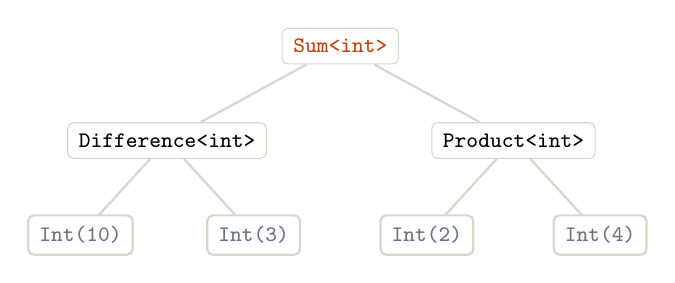
\begin{tikzpicture}[
        font=\ttfamily\footnotesize,
        nd/.style={draw=rule,rounded corners=2pt,inner sep=4pt,fill=white},
        leaf/.style={nd,text=muted},
        level distance=12mm,
        level 1/.style={sibling distance=44mm},
        level 2/.style={sibling distance=22mm},
        edge from parent/.style={draw=rule,thick}
      ]
      \node[nd,text=accent] {Sum<int>}
        child { node[nd] {Difference<int>}
          child { node[leaf] {Int(10)} }
          child { node[leaf] {Int(3)} }
        }
        child { node[nd] {Product<int>}
          child { node[leaf] {Int(2)} }
          child { node[leaf] {Int(4)} }
        };
    \end{tikzpicture}
  \end{center}
  \vspace{0.6em}
  \begin{center}
    \aside{Seven constructors ran. Zero additions, zero multiplications.}
  \end{center}
\end{frame}
\note{The graph is the program, and it is standing still.}

\begin{frame}{Names}
  \vspace{0.8em}
  {\Large We name a component for \handstroke{what it is}, not for what it
  does.}

  \vspace{1.4em}
  \begin{columns}[t,onlytextwidth]
    \begin{column}{0.45\textwidth}
      {\color{accent}\footnotesize YES}\\[0.7em]
      \texttt{ConcatenatedString}\\[0.4em]
      \texttt{Sum}\\[0.4em]
      \texttt{Difference}\\[0.4em]
      \texttt{CurrentTime}
    \end{column}
    \begin{column}{0.45\textwidth}
      {\color{muted}\footnotesize NO}\\[0.7em]
      {\color{muted}\texttt{StringConcatenator}}\\[0.4em]
      {\color{muted}\texttt{Calculate}}\\[0.4em]
      {\color{muted}\texttt{TimeProvider}}
    \end{column}
  \end{columns}

  \vspace{1.5em}
  \aside{A component is not an agent that performs an action --- it is a value
  that stands for one. Read a composition out loud and you are reading a noun
  phrase, not a procedure.}
\end{frame}
\note{It is a rule, not a habit.}

\begin{frame}{So where does it ever end?}
  \vspace{1.1em}
  {\Large It happens at the \handstroke{native field}.}

  \vspace{1.4em}
  The moment somebody reads \texttt{.TextValue} --- or \texttt{.BoolValue}, or
  \texttt{.NumberValue}:

  \vspace{0.9em}
  \begin{itemize}
    \setlength{\itemsep}{0.45em}
    \item the graph is walked,
    \item every deferred operation runs in order,
    \item a concrete .NET value comes out the other side.
  \end{itemize}
\end{frame}
\note{If nothing computes, when does anything happen?}

\begin{frame}[fragile]{``What if I read it twice?'' --- then it runs twice}
  \vspace{0.1em}
\begin{lstlisting}[basicstyle=\ttfamily\scriptsize]
public sealed record CachedString : IString
{
    private readonly Lazy<string> _lazyValue;

    public CachedString(IString value)
        : this(
            new Lazy<string>(
                () => value.TextValue,
                LazyThreadSafetyMode.ExecutionAndPublication
            )
        )
    { }

    private CachedString(Lazy<string> lazyValue)
    {
        _lazyValue = lazyValue;
    }

    public string TextValue => _lazyValue.Value;
}
\end{lstlisting}
  \vspace{0.2em}
  \aside{An \texttt{IString} that holds an \texttt{IString}. Caching is
  \handstroke{one more object in the graph}.}
\end{frame}
\note{A composition keeps no result -- it is a description, and descriptions do
  not remember. Wrapped, the graph is walked exactly once, thread-safely,
  however many reads. And you decide where in the graph it sits.}

% ==================================================== 5. DETERMINED HASH ===
\renewcommand{\sectionclock}{$\approx$ 5.5 min}
\renewcommand{\sectionheadline}{Determined hashes}
\section{Determined hashes}

\begin{frame}[plain]
  \bigline{We use \handstroke{determined hashes} instead of the built-in
    \texttt{GetHashCode} and \texttt{Equals}.}
\end{frame}
\note{Principle five. The one that looked out of place next to the other four.}

\begin{frame}{Why: it is not identity}
  \vspace{0.9em}
  {\Large \texttt{GetHashCode} gives you a different answer the next time you
  run the same program.}

  \vspace{1.4em}
  \begin{itemize}
    \setlength{\itemsep}{0.55em}
    \item Cannot be written to a file.
    \item Cannot be sent over a network.
    \item Cannot be compared to yesterday.
  \end{itemize}

  \vspace{1.1em}
  \aside{The framework's notion of sameness has a lifetime shorter than the
  application's. What we want is the hash of an \textbf{object state
  snapshot}.}
\end{frame}
\note{Deliberate security measure since .NET Core -- not a bug. But identity
  dies with the process.}

\begin{frame}{And a second problem, which is worse}
  \vspace{1.3em}
  \begin{center}
    \Large
    \texttt{0.GetHashCode()} \quad $=$ \quad \texttt{0}\\[0.65em]
    \texttt{false.GetHashCode()} \quad $=$ \quad \texttt{0}\\[0.65em]
    \texttt{default(char).GetHashCode()} \quad $=$ \quad \texttt{0}
  \end{center}
  \vspace{1.6em}
  \begin{center}
    Three different values, from three different types,
    \handstroke{sharing one identity}.
  \end{center}
\end{frame}
\note{Pause on the three zeroes.}

\begin{frame}[fragile]{What we use instead}
  \vspace{0.5em}
\begin{lstlisting}
public interface IDeterminedHash : IEnumerable<byte>;
\end{lstlisting}
  \vspace{0.6em}
  \aside{That is the entire file. An identity is not an integer --- it is a
  \textbf{sequence of bytes}. And it is lazy, like everything else.}

  \vspace{1.2em}
\begin{lstlisting}
public IEnumerator<byte> GetEnumerator()
{
    return SHA256.HashData([.. _bytes]).AsEnumerable().GetEnumerator();
}
\end{lstlisting}
  \vspace{0.6em}
  \aside{SHA-256. Thirty-two bytes. Deterministic across processes, machines
  and runtimes --- which is the entire point.}
\end{frame}
\note{Enumerate it and it computes; leave it alone and it costs nothing.}

\begin{frame}[fragile]{A domain separator per type}
  \vspace{0.7em}
\begin{lstlisting}
private static readonly byte[] TypePrefix =
[
    0, 69, 151, 1, 4, 52, 46, 126, 159, 32, 211, 174, 149, 230, 168, 150,
];
\end{lstlisting}
  \vspace{1.1em}
  Sixteen random bytes, unique per type, prepended before hashing.

  \vspace{0.9em}
  So the number zero, the boolean false and the empty string produce three
  completely different digests.

  \vspace{0.9em}
  \aside{The collision the framework hands you for free is structurally
  impossible here.}
\end{frame}
\note{Every type gets one.}

\begin{frame}{A direct consequence}
  \vspace{0.8em}
  If we do not use \texttt{GetHashCode}, \textbf{we cannot use the framework's
  collections.}

  \vspace{0.9em}
  \aside{A \texttt{Dictionary} or a \texttt{HashSet} asks its keys for a hash
  code, and our objects do not answer that question.}

  \vspace{1.3em}
  \hrulethin{0.5}
  \vspace{1.0em}

  So the ecosystem ships its own collection wrappers, keyed on determined
  hashes. Two keys are the same when their byte sequences are the same.

  \vspace{0.9em}
  The integer underneath has not disappeared --- it is
  \handstroke{demoted from an identity to a bucket index}.
\end{frame}
\note{It no longer answers ``are these the same'', only ``roughly where should I
  look''. Collisions there are harmless, because the real comparison is exact.}

\begin{frame}{One door this opens}
  \vspace{1.5em}
  {\large Objects are immutable, and their state can be determined exactly.}

  \vspace{1.3em}
  So an allocator can ask a different question:

  \vspace{1.0em}
  {\Large \textbf{Has an object with this state already been allocated?}}

  \vspace{1.3em}
  If yes --- there is no need to allocate again. Just return the existing
  reference.

  \vspace{1.2em}
  \aside{Not built. The door is open, and it is only open because of the two
  rules.}
\end{frame}
\note{Mark it as an opportunity, not a claim. Then move on.}

% ======================================================= 6. CONTROL FLOW ===
\renewcommand{\sectionclock}{$\approx$ 5 min}
\renewcommand{\sectionheadline}{Control flow is an object too}
\section{Control flow}

\begin{frame}[plain]
  \bigline{What about \texttt{if}?\\[0.8em]
    {\normalsize\normalfont\color{muted}You cannot compose a keyword. It
    executes, it branches, it does not exist as a value --- and you cannot pass
    it to a constructor.}}
\end{frame}
\note{The question I get in every hallway conversation. And a language without
  branching is not a language.}

\begin{frame}[fragile]{An \texttt{if} that produces a string \emph{is} a string}
  \vspace{0.1em}
\begin{lstlisting}[basicstyle=\ttfamily\scriptsize]
public sealed record StringChoice : IString
{
    private readonly IBool _condition;
    private readonly IString _valueOnTrue;
    private readonly IString _valueOnFalse;

    public StringChoice(IBool condition, IString valueOnTrue, IString valueOnFalse)
    {
        _condition = condition;
        _valueOnTrue = valueOnTrue;
        _valueOnFalse = valueOnFalse;
    }

    public string TextValue =>
        _condition.BoolValue ? _valueOnTrue.TextValue : _valueOnFalse.TextValue;
}
\end{lstlisting}
  \vspace{0.2em}
  \aside{The condition is an object. Both branches are objects. And the choice
  \handstroke{implements the target interface}.}
\end{frame}
\note{It is not a control structure that yields a value. It is a value that
  happens to have a decision inside it.}

\begin{frame}[fragile]{Which means it composes}
  \vspace{0.5em}
\begin{lstlisting}
INumber<int> count = new Int(3);

IString label = new WrappedString(
    new LeftCurlyBracketString(),
    new StringChoice(
        new GreaterThanCondition<int>(count, new Zero<int>()),
        new String(count),
        new EmptyString()
    ),
    new RightCurlyBracketString()
);
\end{lstlisting}
  \vspace{0.8em}
  \aside{The \texttt{WrappedString} has no idea there is a branch inside it. It
  was handed an \texttt{IString}, and that is all it will ever know.}
\end{frame}
\note{A choice inside a concatenation, inside another choice, inside a cache --
  nothing downstream needs to know a decision is in there.}

\begin{frame}[fragile]{When the interface has more than one field}
  \vspace{0.1em}
\begin{lstlisting}[basicstyle=\ttfamily\tiny]
public sealed record DateChoice : IDate
{
    public DateChoice(IBool condition, IDate valueOnTrue, IDate valueOnFalse)
        : this(
            new NumberChoice<ushort>(condition, valueOnTrue.Day, valueOnFalse.Day),
            new NumberChoice<ushort>(condition, valueOnTrue.Month, valueOnFalse.Month),
            new NumberChoice<ushort>(condition, valueOnTrue.Year, valueOnFalse.Year)
        )
    { }

    private DateChoice(INumber<ushort> day, INumber<ushort> month, INumber<ushort> year)
    {
        Day = day;
        Month = month;
        Year = year;
    }

    public INumber<ushort> Day { get; }
    public INumber<ushort> Month { get; }
    public INumber<ushort> Year { get; }
}
\end{lstlisting}
  \vspace{0.2em}
  \aside{The public constructor performs no branching at all --- it composes
  three smaller choices, one per field, and delegates to the private one that
  assigns.}
\end{frame}
\note{The constructor pattern from the previous section, now applied to
  branching.}

\begin{frame}{The \texttt{if} is distributed}
  \vspace{1.1em}
  {\Large There is no single branch point.}

  \vspace{1.3em}
  The decision lives in \textbf{every field of the interface}, and each one is
  decided independently, at the moment it is read.

  \vspace{1.3em}
  \aside{Ask only for the year, and the day is never chosen. That branch never
  happens at all.}

  \vspace{1.5em}
  A statement executes once, in one place, at one time. This is a decision that
  exists in three places and \handstroke{may partially never occur}.
\end{frame}
\note{That is not something a statement can do.}

\begin{frame}[fragile]{And \texttt{switch}?}
  \vspace{0.7em}
  A switch that returns a string implements \texttt{IString}. But it has to
  answer one question the choice never had to: \textbf{is this the same as
  that?}

  \vspace{1.1em}
\begin{lstlisting}
public StringSwitch(
    TSelector parameter,
    IEnumerable<KeyValuePair<TSelector, IString>> branches,
    Func<TSelector, IDeterminedHash> hashFactory
)
\end{lstlisting}
  \vspace{0.9em}
  \aside{And we already know how Pure answers that. Determined hashes.}
\end{frame}
\note{Hold here -- the diagram is next.}

\begin{frame}{The whole machine}
  \vspace{0.6em}
  \begin{center}
    \scalebox{1.12}{%
    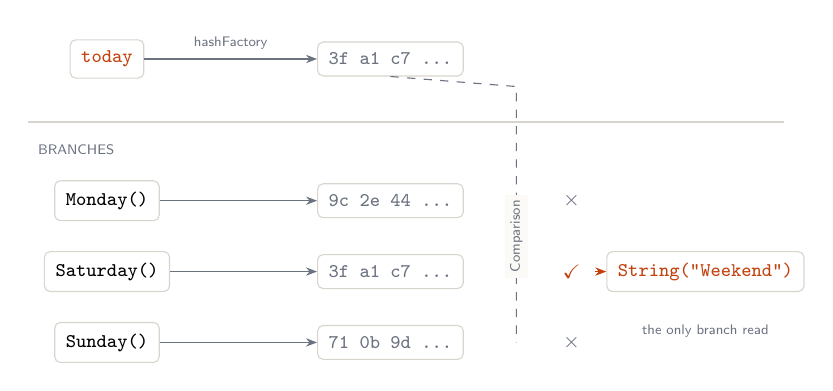
\begin{tikzpicture}[
        font=\ttfamily\scriptsize,
        box/.style={draw=rule,rounded corners=2pt,inner sep=4pt,fill=white},
        hash/.style={box,text=muted},
        arr/.style={-{Stealth[length=4pt]},draw=muted},
        tag/.style={font=\sffamily\tiny,text=muted}
      ]
      % the parameter, hashed
      \node[box,text=accent] (p) at (0,0) {today};
      \node[hash] (ph) at (3.6,0) {3f a1 c7 ...};
      \draw[arr] (p) -- node[tag,above] {hashFactory} (ph);

      \draw[rule] (-1.0,-0.8) -- (8.6,-0.8);
      \node[tag,anchor=west] at (-1.0,-1.15) {BRANCHES};

      % every key, hashed the same way
      \node[box] (b1) at (0,-1.8) {Monday()};
      \node[box] (b2) at (0,-2.7) {Saturday()};
      \node[box] (b3) at (0,-3.6) {Sunday()};

      \node[hash] (h1) at (3.6,-1.8) {9c 2e 44 ...};
      \node[hash] (h2) at (3.6,-2.7) {3f a1 c7 ...};
      \node[hash] (h3) at (3.6,-3.6) {71 0b 9d ...};

      \draw[arr] (b1) -- (h1);
      \draw[arr] (b2) -- (h2);
      \draw[arr] (b3) -- (h3);

      % the comparison
      \draw[draw=muted,dashed] (ph.south) -- (5.2,-0.35) -- (5.2,-3.6);
      \node[tag,rotate=90,fill=paper,inner sep=2pt] at (5.2,-2.25) {Comparison};

      \node[text=muted] at (5.9,-1.8) {$\times$};
      \node[text=accent] at (5.9,-2.7) {$\checkmark$};
      \node[text=muted] at (5.9,-3.6) {$\times$};

      \node[box,text=accent] (res) at (7.6,-2.7) {String("Weekend")};
      \draw[arr,draw=accent] (6.2,-2.7) -- (res);
      \node[tag,anchor=north] at (7.6,-3.25) {the only branch read};
    \end{tikzpicture}}
  \end{center}
\end{frame}
\note{Hash the parameter. Hash each key. Keep the branch whose bytes match, and
  read only that one. The two that lost are still sitting there, unevaluated,
  and they will stay that way.}

\begin{frame}{What is \emph{not} in that picture}
  \vspace{1.4em}
  \begin{center}
    \Large
    No \texttt{==}.\\[0.65em]
    No \texttt{Equals}.\\[0.65em]
    No virtual dispatch to ask an object about itself.
  \end{center}
  \vspace{2.0em}
  \begin{center}
    The switch does not ask the objects whether they are equal.\\[0.8em]
    It is \handstroke{told how to identify them} via a determined state hash.
  \end{center}
\end{frame}
\note{Land this one slowly.}

% ============================================== 7. WHAT IT COSTS AND BUYS ==
\renewcommand{\sectionclock}{$\approx$ 4 min}
\renewcommand{\sectionheadline}{What it costs, and what it buys}
\section{Costs and benefits}

\begin{frame}{The first thing you notice is testing}
  \vspace{1.1em}
  \begin{itemize}
    \setlength{\itemsep}{0.75em}
    \item \textbf{Bounded} --- a component holds exactly the objects it was
          given.
    \item \textbf{Immutable} --- no order of operations to reconstruct, no setup
          to unwind.
    \item \textbf{Thread-safe} by construction.
  \end{itemize}

  \vspace{1.5em}
  {\Large A test becomes what a test should be:
  \handstroke{build, read, compare}.}

  \vspace{0.9em}
  \aside{There is nothing else in the way.}
\end{frame}
\note{This is a headline benefit, not an afterthought.}

\begin{frame}{The cost is at the border}
  \vspace{1.1em}
  {\Large Everything that meets classic .NET needs a wrapper.}

  \vspace{1.4em}
  \aside{An adapter that unwraps an interface into a concrete type on the way
  out, and wraps it back on the way in.}

  \vspace{1.5em}
  \hrulethin{0.5}
  \vspace{1.0em}

  Either you write the adapter, or you implement as much of your domain as
  possible inside the ecosystem, evaluate through a native field at the very
  edge, and carry on from there.

  \vspace{0.8em}
  The further out you push that edge, the fewer adapters you write.
\end{frame}
\note{I would rather tell you the price myself than have someone find it in the
  Q and A.}

\begin{frame}{The objection, stated wrongly}
  \vspace{1.3em}
  \begin{columns}[t,onlytextwidth]
    \begin{column}{0.45\textwidth}
      {\color{muted}\footnotesize TO DESIGN}\\[0.8em]
      {\large It takes \textbf{more} mental power.}\\[0.8em]
      \aside{That part is true.}
    \end{column}
    \begin{column}{0.45\textwidth}
      {\color{accent}\footnotesize TO READ}\\[0.8em]
      {\large Simpler, better, and frankly more satisfying.}\\[0.8em]
      \aside{Than the classic alternative.}
    \end{column}
  \end{columns}

  \vspace{2.0em}
  The difficulty is at the moment of writing --- and it buys clarity every time
  anybody reads it afterwards.
\end{frame}
\note{Do not frame this as a cost the audience must accept.}

\begin{frame}{Seventy-five packages, on purpose}
  \vspace{1.0em}
  One repository per package. One pipeline per package. Not a monolithic SDK.

  \vspace{1.3em}
  \aside{A monolithic SDK forces a decision on you: all of it or none of it. And
  with an idea this opinionated, ``all of it'' is not a reasonable thing to ask
  of anyone.}

  \vspace{1.5em}
  {\Large \handstroke{You do not adopt the ecosystem.}\\[0.5em]
   \handstroke{You take the two packages you need.}}

  \vspace{1.1em}
  \aside{Lazy boolean algebra and nothing else? One package. Deterministic
  hashing in an otherwise conventional codebase? One package --- three lines of
  interface, and no philosophy dragged in behind it.}
\end{frame}
\note{The granularity is only survivable because every repository is generated
  from the same template.}

\begin{frame}[plain]
  \bigline{A program should \emph{be} the transformation\\[0.6em]
    --- written down, composed, and standing there unperformed until someone
    needs it.}
\end{frame}
\note{Finish where I started. Not the interfaces, not the hashes -- those are
  consequences.}

\begin{frame}{At the edges, Pure disappears}
  \vspace{1.3em}
  \begin{center}
    {\large The wire sees a string. The database sees a column. The client sees
    a primitive.}
  \end{center}
  \vspace{1.2em}
  \begin{center}
    \aside{None of them can tell. All of this exists only inside the process,
    between the first constructor and the moment a native field is read.}
  \end{center}
\end{frame}
\note{Slow down -- the last statement is next.}

\begin{frame}[plain]
  \bigline{Your program is a graph of \texttt{new}.\\[0.8em]
    And everything that happens, happens \handstroke{once, at the end} --- when
    somebody finally reads a field.}
\end{frame}
\note{Hold the pause before thanking them.}

\begin{frame}[plain]
  \vfill
  {\Huge\bfseries Thank you}\\[1.2em]
  \hrulethin{0.32}\\[1.2em]
  {\large \texttt{github.com/kudima03} \quad\textbullet\quad NuGet:
  \texttt{Pure.*}}\\[1.7em]
  {\color{muted}Elegant Objects is the work of Yegor Bugaenko.\\
   Pure is an implementation of those ideas for .NET, with some divergences of
   my own.}
  \vfill
\end{frame}
\note{I would be glad to discuss any of it with you.}

\end{document}
